\chapter{GPGPU}
\label{cap:gpgpu}

A seguir é explanado o que vem a ser uma placa gráfica, principalmente seu processador, a GPU. Depois é descrita a motivação para a qual esse hardware foi criado, o por quê ainda é produzido e por que provavelmente continuará. Seguindo são apontadas as diferenças arquiteturais entre uma CPU e uma GPU, vantagens e desvatagens. Na continuação são apresentadas e demonstradas as duas principais linguagens que permitem o acesso a programação genérica na GPGPU a OpenCL e a CUDA, contendo o por quê neste projeto foi escolhido a linguagem CUDA. Por fim são apresentadas aplicações que se utilizam do estado da arte no hardware e software das placas gráficas mais atuais e avançadas.

\section{Placas de vídeo}
  \begin{figure}[!h]
    \centering
    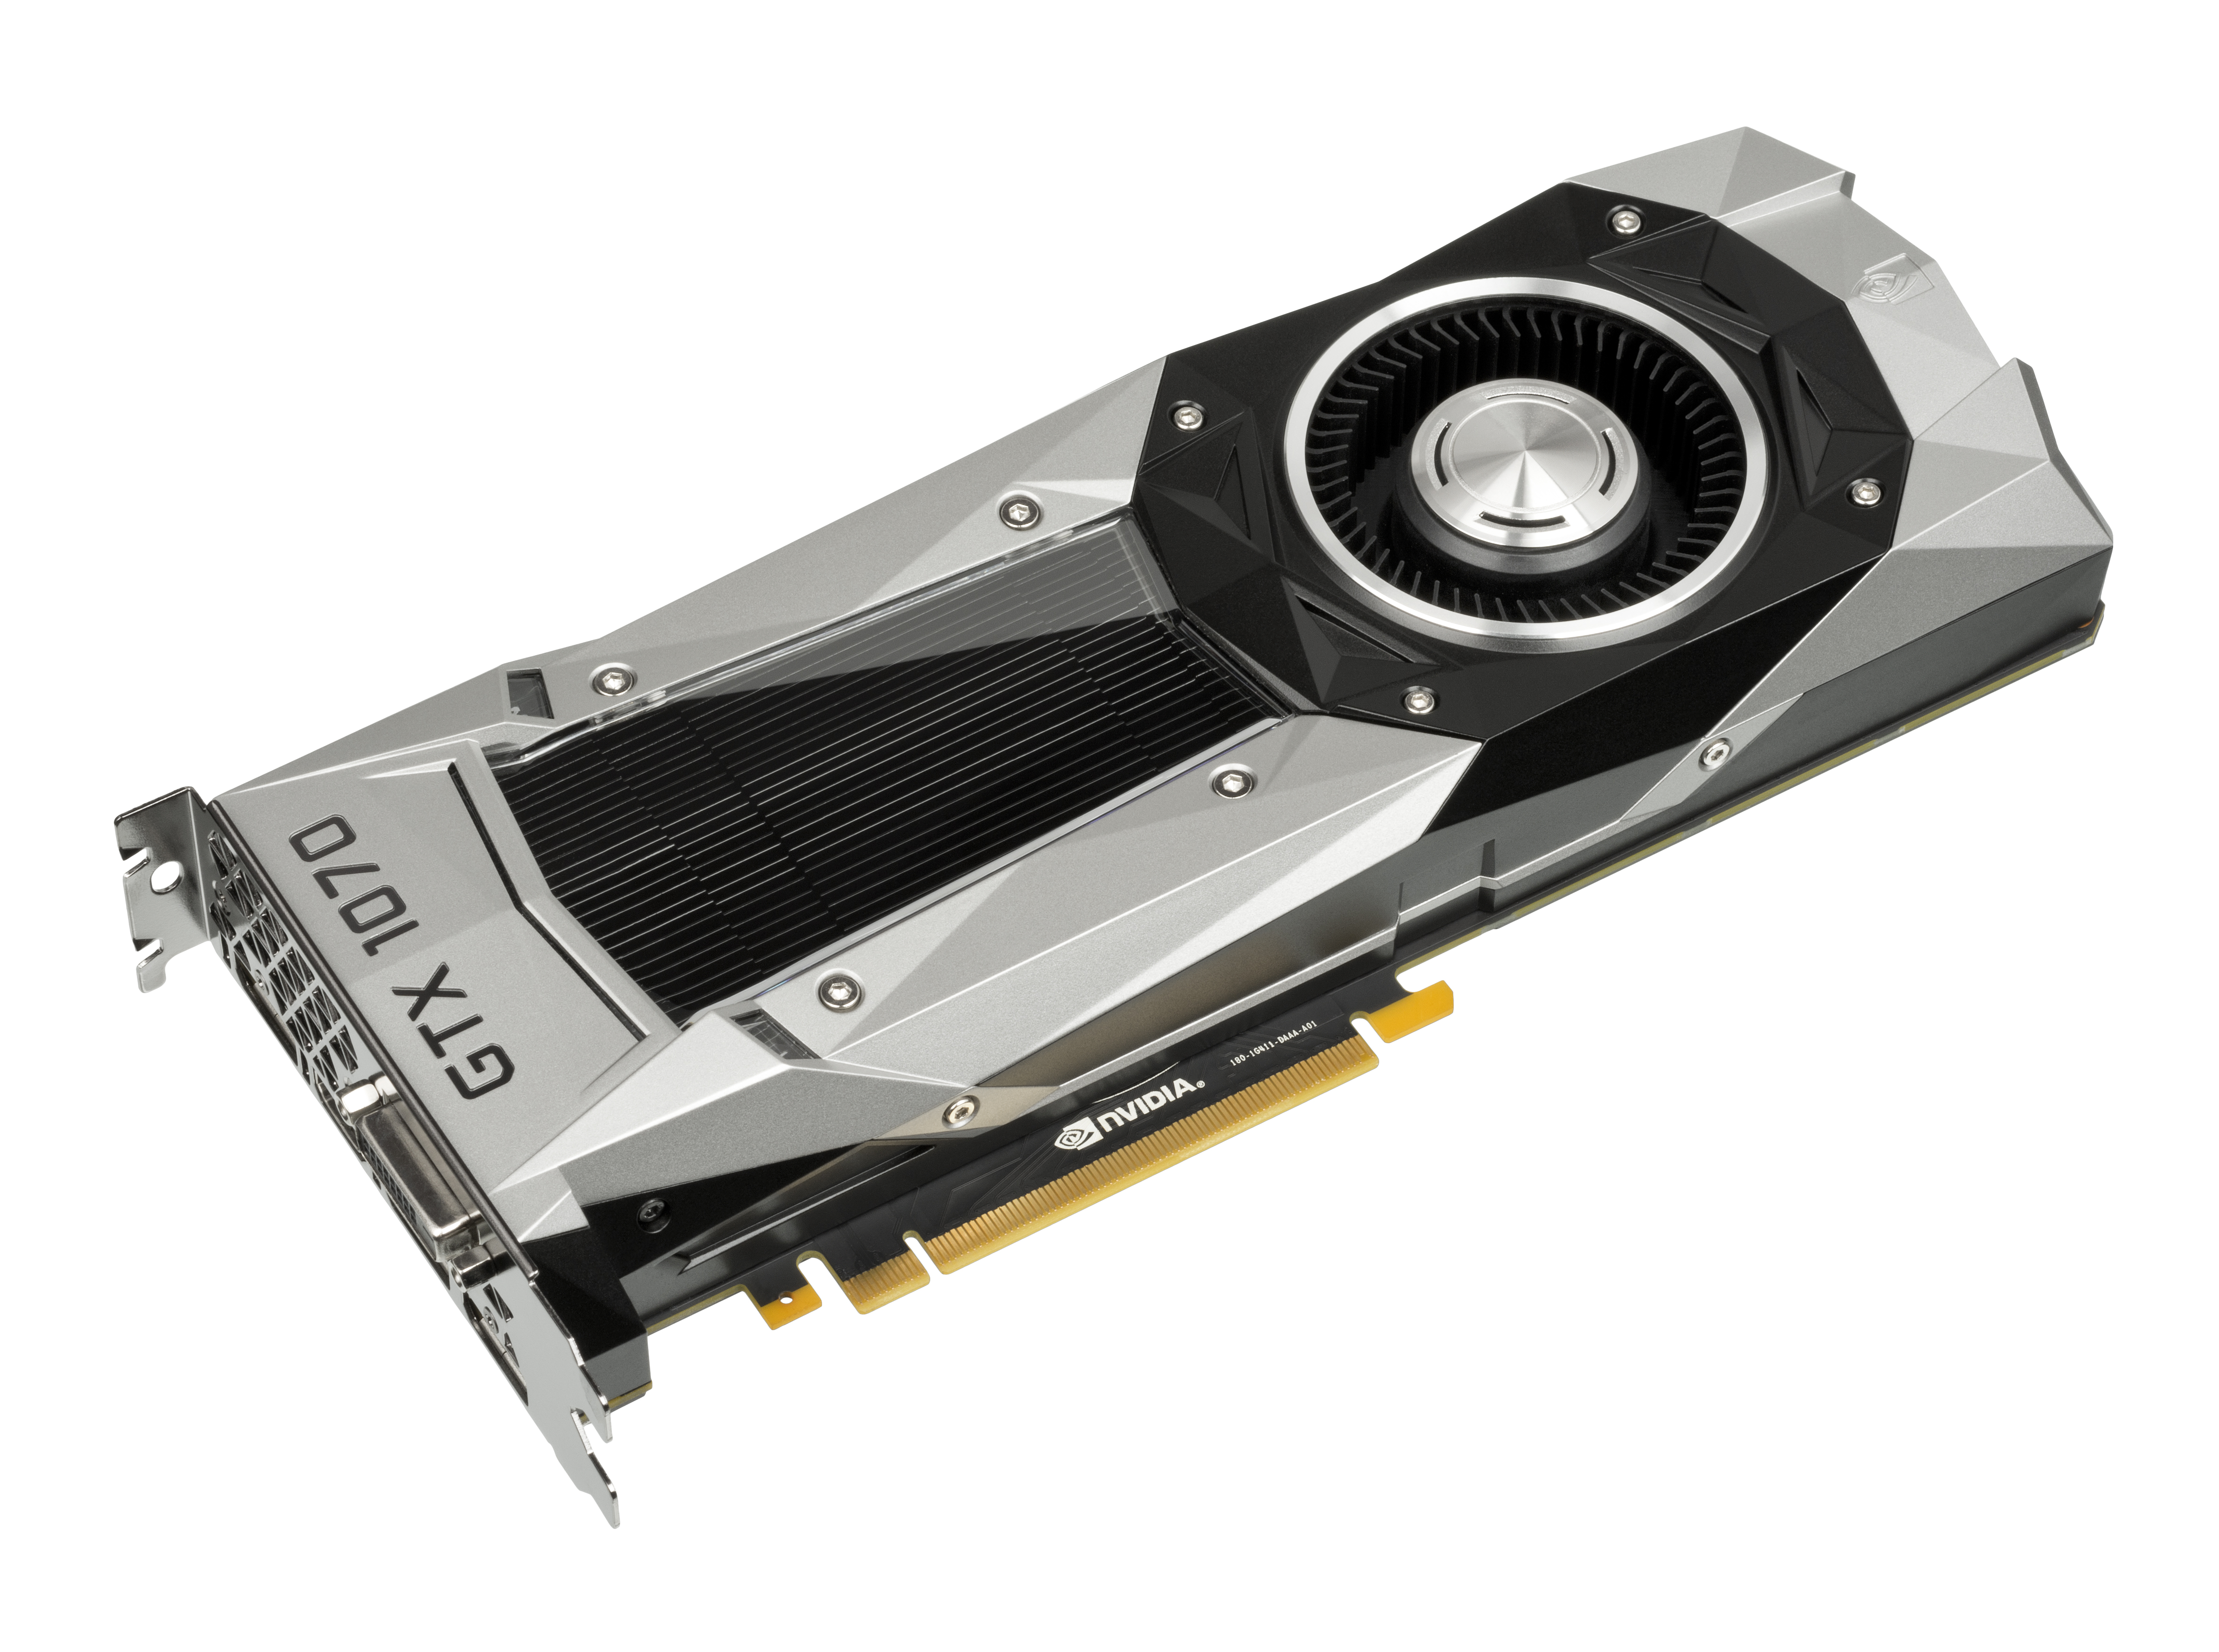
\includegraphics[width=.80\textwidth]{NVIDIA-GTX-1070-FoundersEdition-FL.jpg}
    \caption{Placa grafica NVIDIA GTX 1070 para computadores de mesa "desktop", essa versão é a "Founders edition", possui cerca de 8 GBs de memória com uma banda de 256 GB/s , 1920 núcleos, frequência de funcionamento de 1506 MHz e consome 150W. (Fonte: Wikimedia Commons \protect\footnotemark)}
    \label{fig:gtx1070}
  \end{figure}

  \footnotetext{Disponível em \url{https://commons.wikimedia.org/wiki/File:NVIDIA-GTX-1070-FoundersEdition-FL.jpg} Domínio público}

  Placa de vídeo é uma peça que pode ou não estar presente em um computador, ela é responsável por fornecer o hardware especializado em renderização gráfica, projetado para prover um grande aumento de performance a um baixo custo se comparado a CPUs no que disrespeito a tranformação de dados na memoria em imagens e vídeos, prontos para serem apresentados em telas e monitores. São constituídas principalmente de:
  \begin{itemize}
    \item Um chip de memória, cuja a principal função é armazenar texturas, ou qualquer outro dado que deverá ser várias vezes utilizado, consultado, no processo de renderização.
    \item Portas de acesso e conexão a monitores e telas, variam entre VGA (Video Graphics Array), DVI (Digital Visual Interface) e HDMI (High-Definition Muiltimidia Interface). São as saídas mais comuns às computações das placas.
    \item Um processador, uma GPGPU composta de alguns milhares de núcleos
    \item Uma ou várias ventoinhas, para dissipar o calor produzido pelo processador
  \end{itemize}

  A figura \ref{fig:gtx1070} é uma foto de uma placa gráfica da Nvidia, a NVIDIA GTX 1070, começou a ser comercializada em Junho de 2016 à um preço de 379 dólares e possuí 1920 núcleos de processamento à 1,506 GHz em sua GPU \citep{gtx1070:16}. Nessa mesma época também é comercializada o \textit{Intel® Core™ i7-6850K Processor} CPU da Intel, vendida na época a partir de 617 dólares, possui 6 núcleos à uma frequência de 3,6 GHz \citep{inteli7:16}. Um cálculo simples de tiques por segundo, ou seja, quantidade de ciclos que podem ser executados por segundo para cada processador demonstra que, enquanto a CPU da intel é capaz de realizar 21,6 bilhões de ciclos, no total, por segundo a GPGPU da nvidia é capaz de 2891,52 bilhões de ciclos, no total, por segundo, uma diferença de aproximadamente 133,8 vezes. A GPU que é 60,42\% do valor da CPU é mais de 100 vezes mais rápida.

  GPGPU é uma acrônimo para \textit{General Purpose Graphics Processing Unit} em tradução literal: Unidade de processamento Gráfico de Propósito Geral. É uma evolução, uma adaptação que as GPUs passaram, na qual sua cadeia de processamento gráfico foi flexibilizada tornado possível usá-la para propósitos mais gerais, indo muito além do escopo de produção de gráficos e imagens em três dimensões, porém suas origens e modo de operação advem da sua função original de processar uma cadeia de dados gráficos, e tal necessidade determinou qual seria o objetivo da arquitetura que tais processadores deveriam ter. Assim entender essa cadeia de processamento ou \textit{pipeline} dos dados das placas gráficas é importante para entender o por quê são como são \citep{massively:16}.

  O objetivo das GPUs é gerar imagens e vídeos que representam visões de uma cena virtual. A visão desta cena é descrita pela posição de uma câmera virtual e é definida pela geometria, orientação e propriedades materiais da superfície dos objetos na cena representados, bem como das propiedades das fontes de luz. APIs gráficas como OpenGL \citep{opengl}, DirectX \citep{directx} ou Vulkan\citep{vulkan} representam este processo como um pipeline que executa uma série de operações sobre um conjunto de vértices enviados pela CPU, sendo que cada vértice possui algumas propriedades, tais como cor, posição e vetor normal \citep{closer-look:08}.

  O vertex shader é um programa que executa um conjunto de operações para cada um dos vertíces de entrada, com o intuíto de projetar cada vértice, baseado em sua posição relativa à camera virtual, em um espaço de tela 2D. Destes vértices, é montado um conjunto de triângulos, que representam os objetos no espaço 2D. Assim, quanto maior a quantidade de triângulos, melhor a qualidade com que o objeto será representado \citep{closer-look:08}. Visto que cada cena  possui milhares de vértices e cada um deles pode ser tratado independentemente, os vértices podem ser processados paralelamente \citep{gpu-comp:08}.

  A seguir, ocorre o processo de rasterização, que consiste em determinar quais espaços da tela são cobertos por cada triângulo. Esse processo resulta na geração de fragmentos para cada espaço de tela coberto. Um fragmento é o que virá a ser um pixel, que contem todas as informações necessárias para gerar um na imagem final (profundidade, localização no frame buffer, etc.). A partir da posição da câmera virtual, os fragmentos que são ocultos por outros fragmentos são descartados, só é necessário mostras os objetos que podem ser vistos \citep{gpu-comp:08}.

  Já o pixel shader opera sobre a saída gerada pelo processo de rasterização. O pixel shader é um programa que consiste em um conjunto de operações que são executadas sobre cada fragmento, antes que estes sejam plotados na tela. Utilizando as informações de cor dos vértices e, possivelmente, buscando dados adicionais na memória global em forma de texturas (é nesse momento que a memória principal da placa é necessária), cada fragmento é processado para obter-se a cor final do pixel. Assim como na etapa de processamento de vértices, os fragmentos são independentes e podem ser processados em paralelo. Esta etapa é a que tipicamente demanda maior processamento dentro da estrutura do pipeline gráfico \citep{gpu-comp:08}.

  Uma vez que os programas de shader necessitam ser aplicados em milhares de vértices e pixels independentemente, as GPUs evoluíram para um conjunto de multiprocessadores massivamente paralelos. Além disso, dependendo do balanceamento da carga de trabalho da aplicação, apesar dos pixels serem dependentes dos vértices, ambos podem ser executados paralelamente. Esta característica resultou no aumento da programabilidade dos multiprocessadores da GPU \citep{massively:16}.

  Essa cadeia de processamento é o que destacou as GPUs das CPUs convencionais. No desenvolvimento de processadores dedicados a processar essa cadeia na forma mais eficiente possível as GPUs tomaram um caminho mais focado na paralelização, com mais núcleos, mais unidades logico-aritméticas em detrerimento de mais ciclos por segundo, priorizando uma única memória grande e não muito rápida ao invés de varias camadas de memória cache muito rápida.

  Esta arquiterura muito focada, ganhou a atenção de outras computações não necessariamente ligadas a renderização de imagens. Tal demanda eclodiu na flexibilização das GPUs para GPGPUs.


  intel graphycs



\section{A História das GPU e GPGPU}
  As GPUs, a princípio, não foram criadas para cálculos numéricos ou simulações de particulas e sim para a rederização de imagens para jogos digitais, o alto custo na produção e aquisição de hardware mais potente, pricipalmente a memória, na década de 70 impulsionou a criação de processadores mais dedicados e com funções mais específicas para a rederização gráfica. Impulsionada pelo mercado de jogos de video game, e buscando evitar o alto valor de chips de memória, placas de sistemas de arcade apresentavam uma composição de chips de vídeo para combinar os dados enquanto estes eram escaneados saindo para o monitor \citep{Hague:13}.

  Em 1977 o Atari 2600 usou um \textit{video shifter}, um tipo de circuíto integrado responsável por emitir o sinal de TV, chamado \textit{Television Interface Adaptor} ou TIA. Foi customizado para ser capaz de gerar as imagens finais para a tela, os efeitos sonoros e ler os comandos vindos dos joysticks, teve como direcionamento em seu design a economia de memória RAM, muito cara na época \citep{Hague:13} .
% \citep{atari-field:83}
  Em 1985 o Commodore Amiga apresentou um chip gráfico que vinha com um circuíto \textit{blitter}, para maior velocidade na manipulação de memória, tranformação de bitmaps, desenho de linhas e funções de preenchimento de áreas. Também vinha com um co-pocessador, capaz de executar instruções únicas e manipular os registradores em sincronia com o canhão de desenho dos tubos de raios catódicos das televisões .
  % \citep{amiga:17}

  Na decada de 90 a nintendo e a sony criaram seus consoles de vídeo game, o nintendo 64 e o playstation, ambos capazes de produzir gráficos em 3 dimensões a partir de polígonos. A distição entre os dois principais processadores desses vídeo games eram claras, a nintendo já havia detalhado que seu sistema vinha com dois processadores: um de propositos mais geral o \textit{MIPS R4200} e o \textit{Reality Coprocessor} desenhado para cálculos em 3d de alta performance, audio e vídeo pre-processamento, mapeamento de textura e buferização de profundidade em tempo real .
% \citep{manual64:97} \citep{N64's U.S. Launch}
  A nintendo não utilizou o termo CPU para descrever seu \textit{Reality Coprocessor}, foi a Nvidia em 1999 que popularizou o termo. Ele já existia desde década de 80, porém somente ápos a capanha de marketing de sua placa de vídeo, a GeForce 256 com o logo: \textit{"the world's first GPU"} (A primeira GPU do mundo) que o termo ficou mais comum.

\section{CPU vs GPU}

  \begin{figure}[!h]
    \centering
    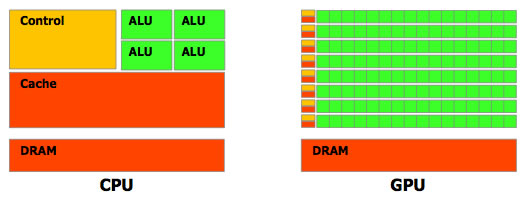
\includegraphics[width=.80\textwidth]{comparacao_GPU_CPU.png}
    \caption{Imagem comparando de forma simplifica a arquitetura dos processadores. Do lado esquerdo a arquitetura de uma Unidade de Processamento Central, muito espaço para o cache e a unidade de comtrole. Do lado direto uma unidade de processamento Gráfica, como uma grande região segmentada dedicada a computação aritimética e lógica. (Fonte: Wikimedia Commons \protect\footnotemark)}
    \label{fig:cpuvsgpu}
  \end{figure}

  \footnotetext{Disponível em \url{https://commons.wikimedia.org/wiki/File:Cpu-gpu.svg} Creative Commons Attribution 3.0 Unported}


  Na Figura~\ref{fig:cpuvsgpu} texto texto

  era uma vez...

\section{Bibliotecas: OpenCL e CUDA}
  o que são e como funcionam
  porque escolhemos cuda?
  colocar código de cada uma

\section{Aplicações e usos avançados}

aprendiozado de máquina, deep learning,
hadoop
simulações climáticas
realidade virtual
renderização em tempo real de rostos humanos reais
bitcoinbilhões de ciclos, no total, por segundo
